% Provenance (never printed): see sources/outline_sources.md (Year 3: the
% Rayleigh number; thermal boundary layers; slab pull and ridge push; plumes;
% post-glacial rebound and mantle viscosity). Brief: sources/book5/BRIEFS.md,
% ch. 6. Curves from figdata/bachelor-3/convection_scaling.py (PREM read only),
% gia_relaxation.py and ridge_push.py (on plate_cooling.py). Exercise and
% problem values in the Book 5 scratch calculator calc/ch06.py.
\chapter{Convection mantellique et forces motrices de la tectonique des plaques}\label{ch:b3:mantle-convection}

La côte du nord de la Suède s'élève hors de la mer d'environ un centimètre par
an, dix mille ans après la fonte de la calotte glaciaire qui la recouvrait~; les
rivages de la baie d'Hudson s'élèvent aussi vite. Rien ne les soulève, sinon le manteau,
qui reflue lentement sous la région que la glace avait enfoncée. La vitesse
à laquelle le sol se redresse dépend de la \omterm{def:b3:mantle-convection:gia}{viscosité du manteau}, et la même
viscosité règle la vitesse de la convection du manteau et le mouvement des plaques. Ce chapitre
cherche à comprendre pourquoi le manteau solide convecte malgré tout, à quelle vitesse il doit s'écouler
pour évacuer la chaleur de la Terre, quelles forces mettent les plaques en mouvement et ce que le rebond du sol
révèle de la \omterm{def:b3:mantle-convection:gia}{viscosité du manteau}.
% ledger: vestol19:umea, zhao12:fenno, sella07:gia

\begin{recall}
La viscosité, l'écoulement rampant d'un fluide visqueux (les équations de Stokes
$\nabla p = \eta\nabla^2\mathbf u$, $\nabla\cdot\mathbf u = 0$), la loi de Stokes
pour une sphère, le nombre de Reynolds et la poussée d'Archimède sont traités dans les
volumes universitaires de physique. La convection mantellique et le rebond isostatique ont été abordés dans le
volume de lycée (niveau~12), la poussée à la dorsale et la traction du panneau plongeant dans sa partie de niveau~11.
La couche limite thermique, la lithosphère thermique et l'adiabate du manteau figurent
dans le volume de première année, dans son chapitre sur le bilan thermique de la Terre~; les points chauds,
les panaches mantelliques et les grandes provinces magmatiques dans son chapitre sur les points chauds.
Le \omterm{def:b3:lithosphere-thermal-models:half-space}{modèle de refroidissement du demi-espace} figure au \cref{ch:b3:lithosphere-thermal-models},
La flexure de la lithosphère figure au \cref{ch:b3:gravity-geodesy}, la
\omterm{def:b3:seismology-imaging:tomography}{tomographie sismique} figure au \cref{ch:b3:seismology-imaging}.
\end{recall}

\section{Pourquoi le manteau convecte}

Le manteau est solide~: il transmet les ondes S. Sur des millions d'années, cependant, il
flue lentement comme un fluide d'énorme viscosité, et une couche de fluide chauffée par
le bas et refroidie par le haut peut rester au repos, la chaleur la traversant par
conduction, ou basculer. Une masse de fluide chaud de taille $d$, plus légère que son
environnement de $\rho\alpha\,\Delta T$, s'élève à une vitesse de
l'ordre de $\rho g\alpha\,\Delta T d^2/\eta$~; elle perd sa chaleur par diffusion en un temps de
l'ordre de $d^2/\kappa$. Si elle peut traverser la couche avant d'avoir refroidi,
la couche bascule.

\begin{definition}[Nombre de Rayleigh]\label{def:b3:mantle-convection:rayleigh}
Pour une couche de fluide d'épaisseur $d$, de masse volumique $\rho$, de coefficient de
dilatation thermique $\alpha$, de diffusivité thermique $\kappa$ et de viscosité $\eta$, sous
la pesanteur $g$, avec un écart de température $\Delta T$ entre sa base et son
sommet, le \emph{nombre de Rayleigh}\index{nombre de Rayleigh} est
\[
  \mathrm{Ra} = \frac{\rho g\alpha\,\Delta T d^3}{\kappa\eta},
\]
le rapport du temps de diffusion $d^2/\kappa$ au temps de montée
par flottabilité $\eta/(\rho g\alpha\,\Delta Td)$.
\end{definition}

\begin{definition}[Nombre de Rayleigh critique]\label{def:b3:mantle-convection:critical}
Le \emph{nombre de Rayleigh critique}\index{nombre de Rayleigh critique}
$\mathrm{Ra}_c$ d'une couche est la valeur du \omterm{def:b3:mantle-convection:rayleigh}{nombre de Rayleigh} au-dessus de laquelle une
petite perturbation de l'état de repos se développe en convection, et en dessous de laquelle
elle s'éteint.
\end{definition}

\begin{proposition}[Déclenchement de la convection]\label{prop:b3:mantle-convection:onset}
Pour une couche dont le sommet et la base sont exempts de contrainte de cisaillement et maintenus à des
températures, une perturbation de nombre d'onde horizontal $k$ (en unités de $1/d$)
croît lorsque $\mathrm{Ra} > (\pi^2 + k^2)^3/k^2$. Le minimum du membre
de droite, atteint en $k = \pi/\sqrt2$, donne
\[
  \mathrm{Ra}_c = \frac{27\pi^4}{4} \approx 657.5,
\]
et les premières cellules à apparaître ont une largeur de $2\sqrt2\,d$. Entre des limites rigides,
$\mathrm{Ra}_c \approx 1708$.
\end{proposition}

\admitted
L'analyse de stabilité linéaire qui la sous-tend, une perturbation des équations de la chaleur et de Stokes
autour de l'état conductif, est traitée dans les volumes de physique
consacrés à la convection~; l'exercice 11 vérifie le minimum.

La figure ci-dessous montre la couche en convection. Les valeurs du manteau, avec la
profondeur de la limite noyau--manteau, $d = \qty{2891}{km}$, la masse volumique moyenne du
manteau, \qty{4476}{kg.m^{-3}}, et $g$ compris entre 9.8 et
\qty{10.7}{m.s^{-2}}, tous issus du modèle sismique terrestre PREM~; $\alpha =
\qty{3.1e-5}{K^{-1}}$ et $\Delta T = \qty{1450}{K}$ tirés du modèle de plaque décrit au
\cref{ch:b3:lithosphere-thermal-models}~; $\kappa = \qty{e-6}{m^2.s^{-1}}$~;
et $\eta$ compris entre \num{e21} et \qty{e22}{Pa.s} (voir la \cref{sec:b3:mantle-convection:gia}),
donnent $\mathrm{Ra}$ compris entre \num{4.9e6} et \num{4.9e7}, soit environ sept mille à
soixante-dix mille fois la valeur critique. Le manteau ne peut pas s'empêcher de convecter.
% ledger: data:prem, honda04:gdh1, delaney86:properties, mitrovica96:haskell, milne04:bifrost

\begin{omfigure}
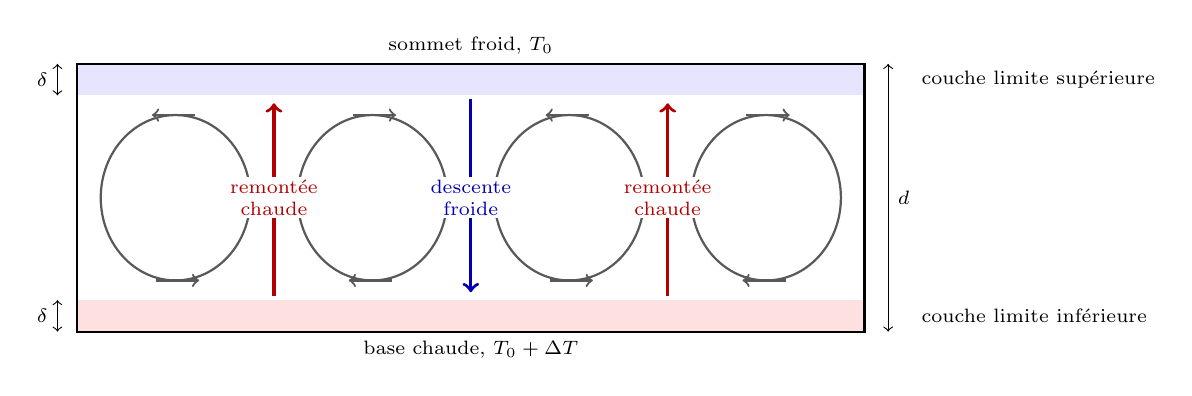
\begin{tikzpicture}[font=\scriptsize, x=1cm, y=1cm]
\fill[blue!10] (0,3.4) rectangle (10,3.0);
\fill[red!12] (0,0) rectangle (10,0.4);
\draw[thick] (0,0) rectangle (10,3.4);
\node[above] at (5,3.4) {sommet froid, $T_0$};
\node[below] at (5,0) {base chaude, $T_0 + \Delta T$};
\foreach \c/\s in {1.25/1, 3.75/-1, 6.25/1, 8.75/-1} {
  \draw[gray!70!black, thick] (\c,1.7) ellipse[x radius=0.95, y radius=1.05];
  \draw[->, gray!70!black, thick] ({\c+0.25*\s},2.75) -- ({\c-0.3*\s},2.75);
  \draw[->, gray!70!black, thick] ({\c-0.25*\s},0.65) -- ({\c+0.3*\s},0.65);
}
\draw[->, red!70!black, very thick] (2.5,0.45) -- (2.5,2.9);
\draw[->, red!70!black, very thick] (7.5,0.45) -- (7.5,2.9);
\draw[->, blue!70!black, very thick] (5,2.95) -- (5,0.5);
\node[red!70!black, fill=white, inner sep=1pt, align=center] at (2.5,1.7) {remontée\\chaude};
\node[red!70!black, fill=white, inner sep=1pt, align=center] at (7.5,1.7) {remontée\\chaude};
\node[blue!70!black, fill=white, inner sep=1pt, align=center] at (5,1.7) {descente\\froide};
\draw[<->] (10.3,0) -- (10.3,3.4) node[midway, right] {$d$};
\draw[<->] (-0.25,3.0) -- (-0.25,3.4) node[midway, left] {$\delta$};
\draw[<->] (-0.25,0) -- (-0.25,0.4) node[midway, left] {$\delta$};
\node[anchor=west] at (10.6,3.2) {couche limite supérieure};
\node[anchor=west] at (10.6,0.2) {couche limite inférieure};
\end{tikzpicture}

\par\smallskip{\small Convection dans une couche chauffée par le bas et refroidie
par le haut. La chaleur traverse les fines couches limites, d'épaisseur $\delta$, par
conduction~; entre les deux, l'intérieur bien mélangé la transporte par écoulement. De
froides lames se détachent de la couche supérieure et s'enfoncent~; les chaudes montent depuis la
couche inférieure.}\label{fig:b3:mantle-convection:cell}
\end{omfigure}

Le manteau est aussi chauffé de l'intérieur, par la désintégration des éléments radioactifs,
et par le bas, par le noyau. Une couche chauffée uniquement de l'intérieur n'a pas de
couche limite à sa base~: son écoulement est mû par de froides lames qui s'enfoncent depuis le
sommet, la remontée étant un retour large et passif. Les panneaux plongeants sont de telles lames, et
les panaches ont besoin de la chaleur venue du noyau.

\section{Couches limites et intensité de la convection}

\begin{definition}[Nombre de Nusselt]\label{def:b3:mantle-convection:nusselt}
Le \emph{nombre de Nusselt}\index{nombre de Nusselt} d'une couche en convection est le
flux de chaleur qui la traverse divisé par le flux que la seule conduction transporterait
à travers la même couche, $\mathrm{Nu} = q\,d/(k\,\Delta T)$.
\end{definition}

\begin{theorem}[Loi d'échelle de couche limite de la convection]\label{thm:b3:mantle-convection:scaling}
Dans une couche en convection à $\mathrm{Ra} \gg \mathrm{Ra}_c$, si chaque couche limite thermique
croît jusqu'à ce que son propre \omterm{def:b3:mantle-convection:rayleigh}{nombre de Rayleigh}, construit sur son épaisseur
$\delta$ et la chute de température $\Delta T/2$ à travers elle, atteigne
$\mathrm{Ra}_c$, alors
\[
  \delta = d\Bigl(\frac{2\mathrm{Ra}_c}{\mathrm{Ra}}\Bigr)^{1/3},\qquad
  \mathrm{Nu} = \frac12\Bigl(\frac{\mathrm{Ra}}{2\mathrm{Ra}_c}\Bigr)^{1/3},
  \qquad
  u = \frac\kappa d\Bigl(\frac{\mathrm{Ra}}{2\mathrm{Ra}_c}\Bigr)^{2/3},
\]
où $u$ est l'échelle de vitesse de l'écoulement, définie en exigeant que la
couche croisse jusqu'à $\delta$ pendant que le fluide traverse la cellule. C'est la
\emph{loi d'échelle de couche limite de la convection}\index{loi d'échelle de couche limite de la convection}.
\end{theorem}

\begin{proof}
L'intérieur est bien mélangé, à la température moyenne, si bien que chaque couche limite
porte la moitié de $\Delta T$. Son \omterm{def:b3:mantle-convection:rayleigh}{nombre de Rayleigh} vaut $\rho g\alpha(\Delta T/2)
\delta^3/(\kappa\eta) = \mathrm{Ra}\,(\delta/d)^3/2$~; en l'égalant à
$\mathrm{Ra}_c$ donne $\delta$. Le flux de chaleur est conduit à travers la couche,
$q = k(\Delta T/2)/\delta$, d'où $\mathrm{Nu} = qd/(k\Delta T) = d/(2\delta)$.
Une couche limite croît par diffusion jusqu'à l'épaisseur $\delta$ en un temps
$\delta^2/\kappa$~; le fluide au sommet traverse la cellule, de largeur de l'ordre de
$d$, en un temps $d/u$. En égalant les deux temps, $u = \kappa d/\delta^2 =
(\kappa/d)(d/\delta)^2$.
\end{proof}

Le flux de chaleur ne croît que comme la racine cubique de $\mathrm{Ra}$~: une viscosité cent fois
plus faible, moins de cinq fois plus de chaleur.
Pour le manteau, où $\mathrm{Ra} = \num{4.9e7}$, la loi donne $\delta \approx \qty{87}{km}$,
$\mathrm{Nu} \approx 17$, un flux de chaleur de $\mathrm{Nu}\,k\Delta T/d \approx
\qty{26}{mW.m^{-2}}$ avec $k = \qty{3.1}{W.m^{-1}.K^{-1}}$, et $u \approx
\qty{1.2}{cm/an}$ (figure ci-dessous). La couche limite est aussi épaisse que la
plaque océanique du \cref{ch:b3:lithosphere-thermal-models}, \qty{95}{km}~; les
\omterm{def:b3:exploration-seismology:velocities}{vitesses quadratiques moyennes} des plaques actuelles vont de \qty{1.1}{cm/an} (Amérique du
Sud) à \qty{7.5}{cm/an} (plaque de Cocos), \qty{4.4}{cm/an} pour l'ensemble de la
lithosphère. Le flux de chaleur moyen de la Terre, \qty{92}{mW.m^{-2}}, vaut trois à quatre
fois celui de la loi~: la chaleur produite dans le manteau, que laisse de côté une couche
chauffée par le bas, et les constantes d'ordre un que la loi
ignore pèsent toutes deux. Pour une loi à une seule donnée, les ordres de grandeur
sont justes~: les plaques sont la couche limite supérieure d'un manteau de $\mathrm{Ra}
\sim 10^7$.
% ledger: nnr56:rms, b2dd10:continents, honda04:gdh1

\begin{omfigure}
\begin{tikzpicture}
\begin{groupplot}[group style={group size=1 by 2, vertical sep=2.5cm},
  omrecord, width=0.86\linewidth, height=0.40\linewidth, xmode=log, ymode=log,
  xmin=100, xmax=1e10, xlabel={Nombre de Rayleigh $\mathrm{Ra}$}]
\nextgroupplot[ylabel={Nombre de Nusselt}, ymin=0.3, ymax=300,
  title={(a) flux de chaleur, en unités du flux conductif}, title style={font=\small}]
% computed in figdata/bachelor-3/convection_scaling.py; ledger: data:prem, honda04:gdh1
\addplot[omDef, thick] table[x=ra, y=nu] {figdata/out/bachelor-3-convection_scaling-conduction.dat};
\addplot[red!70!black, thick] table[x=ra, y=nu] {figdata/out/bachelor-3-convection_scaling-scaling.dat};
\addplot[gray, densely dashed, unbounded coords=jump] table[x=ra, y=y] {figdata/out/bachelor-3-convection_scaling-band.dat};
\draw[gray, densely dotted] (axis cs:657.5,0.3) -- (axis cs:657.5,1);
\node[font=\scriptsize, anchor=west] at (axis cs:700,0.45) {$\mathrm{Ra}_c$};
\node[font=\scriptsize, anchor=south west, omDef] at (axis cs:115,1.08) {conduction};
\node[font=\scriptsize, anchor=north west, red!70!black] at (axis cs:3e4,0.95) {$\tfrac12(\mathrm{Ra}/2\mathrm{Ra}_c)^{1/3}$};
\node[font=\scriptsize, fill=white, inner sep=1pt] at (axis cs:1.55e7,120) {manteau};
\nextgroupplot[ylabel={vitesse (\unit{cm/an})}, ymin=1e-3, ymax=100,
  title={(b) échelle de vitesse pour $d = \qty{2891}{km}$}, title style={font=\small}]
\addplot[red!70!black, thick] table[x=ra, y=u] {figdata/out/bachelor-3-convection_scaling-scaling.dat};
\addplot[gray, densely dashed, unbounded coords=jump] table[x=ra, y=y] {figdata/out/bachelor-3-convection_scaling-band.dat};
\addplot[blue!70, thick, dash dot, unbounded coords=jump] table[x=ra, y=u] {figdata/out/bachelor-3-convection_scaling-plates.dat};
\node[font=\scriptsize, anchor=south west, blue!60!black] at (axis cs:150,7.6) {plaque la plus rapide};
\node[font=\scriptsize, anchor=north west, blue!60!black] at (axis cs:150,1.0) {plaque la plus lente};
\node[font=\scriptsize, fill=white, inner sep=1pt] at (axis cs:1.55e7,0.004) {manteau};
\end{groupplot}
\end{tikzpicture}

\par\smallskip{\small Loi d'échelle de la convection. (a) Sous $\mathrm{Ra}_c$, la couche
conduit la chaleur ($\mathrm{Nu} = 1$)~; loin au-dessus, la loi de couche limite, tracée
à partir de $\mathrm{Ra} = 16\,\mathrm{Ra}_c \approx \num{1.1e4}$, où elle donne $\mathrm{Nu} = 1$ (entre les deux,
la convection s'installe progressivement). (b) L'échelle de vitesse
pour la profondeur du manteau et $\kappa = \qty{e-6}{m^2.s^{-1}}$, avec la
plage des vitesses actuelles des plaques (en tiret-point). Les lignes en tirets encadrent le \omterm{def:b3:mantle-convection:rayleigh}{nombre de
Rayleigh} du manteau pour des viscosités de \num{e22} et \qty{e21}{Pa.s}.}\label{fig:b3:mantle-convection:scaling}
\end{omfigure}

\section{Les forces sur une plaque}

Une plaque se déplace à vitesse stationnaire~: les forces qui s'exercent sur elle se compensent. Trois la poussent ou la
retiennent par ses bords et sa base (figure ci-dessous). La force que
le panneau plongeant exerce sur sa plaque, la traction du panneau plongeant, provient de l'excès de
densité d'une lame froide dans le manteau plus chaud. La poussée à la dorsale, c'est-à-dire la
poussée exercée par la dorsale haute et chaude sur la plaque voisine plus froide, découle du \omterm{def:b3:lithosphere-thermal-models:half-space}{modèle de refroidissement du demi-espace}
du \cref{ch:b3:lithosphere-thermal-models}.

\begin{omfigure}
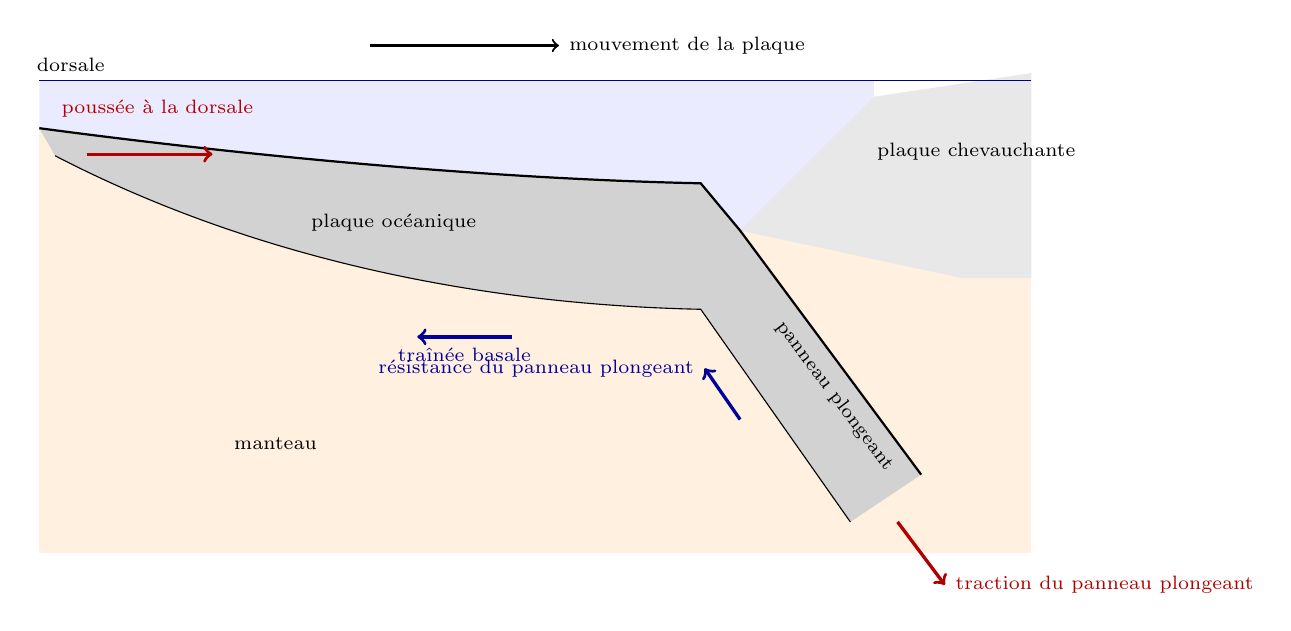
\begin{tikzpicture}[font=\scriptsize, x=1cm, y=1cm]
\fill[orange!12] (0,-0.6) rectangle (12.6,-6.0);
\fill[blue!8] (0,0) -- (0,-0.6) .. controls (3,-1.0) and (6,-1.25) .. (8.4,-1.3) -- (8.9,-1.9) -- (10.6,-0.2) -- (10.6,0) -- cycle;
\fill[gray!35] (0,-0.6) .. controls (3,-1.0) and (6,-1.25) .. (8.4,-1.3) -- (8.9,-1.9) -- (11.2,-5.0) -- (10.3,-5.6) -- (8.4,-2.9) .. controls (6,-2.85) and (3,-2.4) .. (0.2,-0.95) -- cycle;
\fill[gray!18] (10.6,-0.2) -- (12.6,0.1) -- (12.6,-2.5) -- (11.7,-2.5) -- (8.9,-1.9) -- cycle;
\draw[thick] (0,-0.6) .. controls (3,-1.0) and (6,-1.25) .. (8.4,-1.3) -- (8.9,-1.9) -- (11.2,-5.0);
\draw (0.2,-0.95) .. controls (3,-2.4) and (6,-2.85) .. (8.4,-2.9) -- (10.3,-5.6);
\draw[blue!50!black] (0,0) -- (12.6,0);
\node at (0.4,0.2) {dorsale};
\node at (4.5,-1.8) {plaque océanique};
\node at (11.9,-0.9) {plaque chevauchante};
\node[rotate=-53] at (10.1,-4.0) {panneau plongeant};
\node at (3,-4.6) {manteau};
\draw[->, very thick, red!70!black] (0.6,-0.93) -- (2.2,-0.93);
\node[red!70!black] at (1.5,-0.35) {poussée à la dorsale};
\draw[->, very thick, red!70!black] (10.9,-5.6) -- (11.5,-6.4) node[right] {traction du panneau plongeant};
\draw[->, very thick, blue!60!black] (6.0,-3.25) -- (4.8,-3.25) node[below, pos=0.5] {traînée basale};
\draw[->, very thick, blue!60!black] (8.9,-4.3) -- (8.45,-3.65) node[left] {résistance du panneau plongeant};
\draw[->, thick] (4.2,0.45) -- (6.6,0.45) node[right] {mouvement de la plaque};
\end{tikzpicture}

\par\smallskip{\small Les forces sur une plaque océanique~: poussée à la dorsale et traction du panneau plongeant
la poussent (en rouge)~; la traînée à sa base, là où la plaque avance plus vite que le manteau
qui se trouve dessous, et la résistance visqueuse du manteau au panneau plongeant
la freinent (en bleu).}\label{fig:b3:mantle-convection:forces}
\end{omfigure}

\begin{proposition}[Force de poussée à la dorsale]\label{prop:b3:mantle-convection:ridge-push}
Dans le \omterm{def:b3:lithosphere-thermal-models:half-space}{modèle de refroidissement du demi-espace}, avec une température du manteau $T_m$, une température de surface
$T_0$ et une compensation isostatique, la force horizontale par unité
de longueur de dorsale que la colonne à la dorsale exerce sur la plaque d'âge $t$,
la \emph{force de poussée à la dorsale}\index{force de poussée à la dorsale}, vaut
\[
  F_{rp} = g\rho_m\alpha(T_m - T_0)\kappa t\Bigl[1 + \frac{2\rho_m\alpha(T_m
  - T_0)}{\pi(\rho_m - \rho_w)}\Bigr].
\]
\end{proposition}

\begin{proof}
Soient $y$ la profondeur sous le plancher océanique à la dorsale, $w$ l'affaissement du
plancher d'âge $t$, $\theta(z) = T_m - T(z)$ le déficit de température à la
profondeur $z = y - w$ dans sa plaque, et $\Theta(z) = \int_0^z\theta$. La
colonne à la dorsale contient du manteau de masse volumique $\rho_m$ depuis $y = 0$~; la
colonne ancienne contient de l'eau jusqu'à $w$, puis de la plaque de masse volumique $\rho_m(1 + \alpha\theta)$. Les
pressions lithostatiques diffèrent de $P_r - P_t = (\rho_m - \rho_w)gy$ pour $y < w$,
et, plus bas,
\[
  P_r - P_t = (\rho_m - \rho_w)gw - \rho_mg\alpha\,\Theta(z)
  = \rho_mg\alpha\bigl(\Theta(\infty) - \Theta(z)\bigr),
\]
par isostasie, $(\rho_m - \rho_w)w = \rho_m\alpha\Theta(\infty)$. La force est
l'intégrale de la différence de pression sur la profondeur~; en intégrant la seconde partie par
parties,
\[
  F_{rp} = \tfrac12(\rho_m - \rho_w)gw^2 + \rho_mg\alpha\int_0^\infty
  z\,\theta(z)\,\mathrm dz .
\]
Pour le demi-espace, $\theta = (T_m - T_0)\operatorname{erfc}(z/2\sqrt{\kappa
t})$ et $\int_0^\infty x\operatorname{erfc}x\,\mathrm dx = 1/4$, si bien que
l'intégrale vaut $(T_m - T_0)\kappa t$~; et $w = 2\rho_m\alpha(T_m -
T_0)\sqrt{\kappa t/\pi}/(\rho_m - \rho_w)$. En additionnant les deux termes, on obtient la
formule.
\end{proof}

La poussée à la dorsale croît linéairement avec l'âge~: ce n'est pas une poussée à l'axe mais un
gradient de pression réparti sur toute la plaque en refroidissement. Avec les valeurs
du \cref{ch:b3:lithosphere-thermal-models}, le crochet vaut 1.04 et $F_{rp} =
\qty{3.8e12}{N.m^{-1}}$ à \qty{100}{Ma}. Dans le modèle de plaque, elle cesse de croître
avec la profondeur, vers \qty{2.3e12}{N.m^{-1}} (figure ci-dessous). La traction du panneau plongeant est
plus grande~: un panneau de \qty{95}{km} d'épaisseur, en moyenne plus froid de $(T_m - T_0)/2$ que le
manteau, donc plus dense de $\rho_m\alpha(T_m - T_0)/2 \approx
\qty{74}{kg.m^{-3}}$, descendant jusqu'à \qty{670}{km}, pèse
\qty{4.6e13}{N.m^{-1}} de plus que le manteau qu'il déplace, soit douze fois la
poussée à la dorsale. Une grande part de ce poids est absorbée par le manteau visqueux qui résiste à
l'enfoncement du panneau, et seule une partie atteint la plaque.
% ledger: honda04:gdh1, data:prem

\begin{omfigure}
\begin{tikzpicture}
\begin{axis}[omrecord, width=0.8\linewidth, height=0.42\linewidth,
  xmin=0, xmax=160, ymin=0, ymax=6.5, xlabel={âge du plancher océanique (Ma)},
  ylabel={$F_{rp}$ (\qty{e12}{N.m^{-1}})},
  legend cell align=left,
  legend style={font=\scriptsize, at={(0.03,0.97)}, anchor=north west}]
% computed in figdata/bachelor-3/ridge_push.py; ledger: honda04:gdh1
\addplot[omDef, thick] table[x=t, y=hs] {figdata/out/bachelor-3-ridge_push-force.dat};
\addlegendentry{demi-espace}
\addplot[red!70!black, thick, densely dashed] table[x=t, y=pl] {figdata/out/bachelor-3-ridge_push-force.dat};
\addlegendentry{plaque, $L = \qty{95}{km}$}
\end{axis}
\end{tikzpicture}

\par\smallskip{\small \omterm{prop:b3:mantle-convection:ridge-push}{Force de poussée à la dorsale} en fonction de l'âge de la plaque, issue des
deux modèles de refroidissement du \cref{ch:b3:lithosphere-thermal-models}, par intégration numérique
de la différence de pression (la courbe du demi-espace est la forme
fermée de la proposition).}\label{fig:b3:mantle-convection:ridge-push}
\end{omfigure}

\begin{definition}[Traînée basale]\label{def:b3:mantle-convection:basal-drag}
\emph{traînée basale}\index{traînée basale} est la force de cisaillement par unité de surface que le
manteau sous une plaque exerce sur la base de celle-ci. Pour une plaque se déplaçant à la vitesse $u$
au-dessus d'une couche d'épaisseur $h$ et de viscosité $\eta$ dont la base est immobile, elle vaut
$\eta u/h$, dirigée à l'opposé du mouvement~; elle entraîne la plaque là où le manteau sous-jacent
se déplace plus vite qu'elle.
\end{definition}

On peut lire quelles forces comptent à partir des plaques elles-mêmes. Le bilan des couples
sur chaque plaque, ajusté aux mouvements des plaques, indique que les forces agissant sur le
panneau plongeant contrôlent la vitesse des plaques océaniques et sont environ dix fois
plus fortes que toutes les autres, et que la résistance à la base est plus grande sous
les continents que sous les océans. Les vitesses concordent~: les plaques les plus rapides, Cocos à
\qty{75}{mm/an}, Nazca à 70 et le Pacifique à \qty{66}{mm/an}, sont des plaques océaniques
dont les bords plongent dans de longues fosses~; les plus lentes portent de grands continents,
Eurasie à 23, Amérique du Nord à 20, Amérique du Sud à \qty{11}{mm/an}.
% ledger: fu75:slab-pull, nnr56:rms

\section{Panaches}

Des nappes chaudes qui montent de la base du manteau se rassemblent en colonnes~: les panaches
mantelliques du volume de première année, avec une grosse tête et une queue fine (figure ci-dessous).
Le bombement d'un point chaud, une large élévation du fond marin autour des volcans et en aval de
ceux-ci, mesure la quantité de flottabilité qu'apporte son panache.

\begin{definition}[Flux de flottabilité du panache]\label{def:b3:mantle-convection:buoyancy-flux}
Le \emph{flux de flottabilité du panache}\index{flux de flottabilité du panache} $B$ est le
déficit de masse, par rapport au manteau environnant, qu'un panache transporte vers le haut par
unité de temps~; pour un panache de flux volumique $Q_v$ et d'excès de température $\Delta T$,
$B = \rho\alpha\,\Delta T\,Q_v$.
\end{definition}

\begin{proposition}[Flux de flottabilité déduit d'un bombement]\label{prop:b3:mantle-convection:swell}
Si une plaque se déplaçant à la vitesse $u$ au-dessus d'un panache porte un bombement de
section transversale $A$ en travers de la trace, soutenu isostatiquement par le
matériau du panache situé en dessous, le \omterm{def:b3:mantle-convection:buoyancy-flux}{flux de flottabilité du panache} est
\[
  B = (\rho_m - \rho_w)\,A\,u .
\]
\end{proposition}

\begin{proof}
Par isostasie, une tranche de bombement de longueur unitaire le long de la trace, qui soulève
le fond marin sur l'aire $A$ de la section transversale et remplace l'eau par
de la roche, est soutenue par un déficit de masse $(\rho_m - \rho_w)A$ dans la colonne située en dessous.
La plaque emporte la tranche à la vitesse $u$, donc en état stationnaire le
panache doit fournir le déficit correspondant à une longueur $u$ de nouveau bombement par unité de temps.
\end{proof}

À partir des sections transversales des bombements, les flux de flottabilité des points chauds s'étendent sur
un facteur vingt~: Hawaï, le plus grand, \qty{8.7}{Mg/s}~; Islande
\qty{1.4}{Mg/s}~; 37 points chauds réunis, environ \qty{50}{Mg/s}. Chaque kilogramme de
flottabilité représente $c_p/\alpha$ joules de chaleur en excès, donc le flux de chaleur vaut $c_pB/\alpha$~;
avec $c_p = k/(\rho_m\kappa) = \qty{1170}{J.kg^{-1}.K^{-1}}$ et $\alpha =
\qty{3.1e-5}{K^{-1}}$, les 37 points chauds transportent environ \qty{1.9}{TW}, soit
\qty{3.7}{mW.m^{-2}} répartis sur la surface terrestre de \qty{5.1e14}{m^2}, proche de la
\qty{4}{mW.m^{-2}} publié avec les flux~: quelques pour cent de la
\qty{47}{TW} que perd la Terre. Les panaches sont le partenaire secondaire du
bilan thermique~; les plaques transportent le reste.
% ledger: sleep90:flux, b2dd10:half-space, honda04:gdh1

\begin{omfigure}
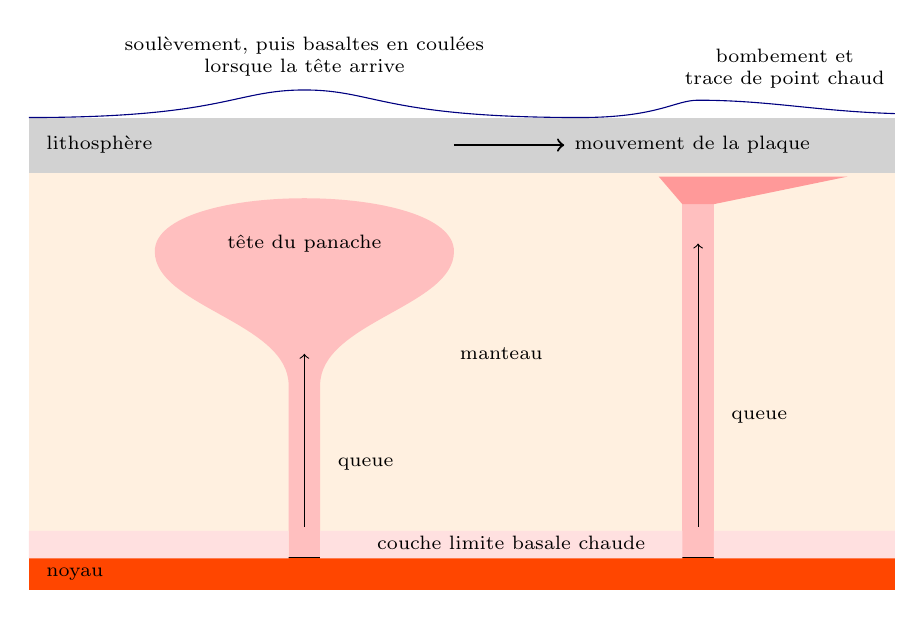
\begin{tikzpicture}[font=\scriptsize, x=1cm, y=1cm]
\fill[orange!12] (0,0) rectangle (11,-5.6);
\fill[gray!35] (0,0) -- (11,0) -- (11,-0.7) -- (0,-0.7) -- cycle;
\fill[red!25] (3.3,-5.6) -- (3.3,-3.4) .. controls (3.3,-2.6) and (1.6,-2.4) .. (1.6,-1.7)
  .. controls (1.6,-0.8) and (5.4,-0.8) .. (5.4,-1.7) .. controls (5.4,-2.4) and (3.7,-2.6) .. (3.7,-3.4) -- (3.7,-5.6) -- cycle;
\fill[red!25] (8.3,-5.6) -- (8.3,-0.75) -- (8.7,-0.75) -- (8.7,-5.6) -- cycle;
\fill[red!40] (8.0,-0.75) -- (8.3,-1.1) -- (8.7,-1.1) -- (10.4,-0.75) -- cycle;
\draw[thick] (0,-5.6) -- (11,-5.6);
\fill[red!45!orange] (0,-5.6) rectangle (11,-6.0);
\fill[red!12] (0,-5.6) rectangle (3.3,-5.25) (3.7,-5.6) rectangle (8.3,-5.25) (8.7,-5.6) rectangle (11,-5.25);
\node[anchor=west] at (0.1,-5.8) {noyau};
\node at (3.5,-1.6) {tête du panache};
\node[anchor=west] at (3.8,-4.4) {queue};
\node[anchor=west] at (8.8,-3.8) {queue};
\node[anchor=west] at (0.1,-0.35) {lithosphère};
\node at (6.0,-3.0) {manteau};
\draw[->] (3.5,-5.2) -- (3.5,-3.0);
\draw[->] (8.5,-5.2) -- (8.5,-1.6);
\draw[->, thick] (5.4,-0.35) -- (6.8,-0.35) node[right] {mouvement de la plaque};
\draw[blue!50!black] (0,0) .. controls (2.5,0) and (2.6,0.35) .. (3.5,0.35) .. controls (4.4,0.35) and (4.5,0) .. (7,0) .. controls (8,0) and (8.2,0.22) .. (8.5,0.22) .. controls (9.4,0.22) and (10,0.08) .. (11,0.05);
\node[above, align=center] at (3.5,0.4) {soulèvement, puis basaltes en coulées\\lorsque la tête arrive};
\node[above, align=center] at (9.6,0.25) {bombement et\\trace de point chaud};
\node[anchor=west] at (4.3,-5.4) {couche limite basale chaude};
\end{tikzpicture}

\par\smallskip{\small Un jeune panache (à gauche) monte sous forme d'une grosse tête alimentée par une fine
queue~; lorsque la tête s'étale sous la lithosphère, la surface se soulève et de grandes
coulées basaltiques peuvent faire éruption. Un panache plus ancien (à droite) est une queue située sous une plaque en mouvement,
qui alimente un bombement et une trace de point chaud. Pas à
l'échelle.}\label{fig:b3:mantle-convection:plume}
\end{omfigure}

Une tête de panache est une sphère de manteau flottant qui monte à travers le manteau visqueux~:
la loi de Stokes vue en physique, $v = 2\Delta\rho\,ga^2/(9\eta)$, donne sa vitesse à l'ordre de
grandeur, une fraction de mètre par an pour une tête de quelques centaines de kilomètres
de diamètre (exercice 8), de sorte qu'elle traverse le manteau en millions d'années.

\section{Ajustement isostatique glaciaire et viscosité du manteau}\label{sec:b3:mantle-convection:gia}

\begin{definition}[Ajustement isostatique glaciaire, viscosité du manteau]\label{def:b3:mantle-convection:gia}
\emph{ajustement isostatique glaciaire}\index{ajustement isostatique glaciaire} (GIA)
est la lente déformation de la Terre solide, ainsi que la variation de son champ
de gravité et du niveau de la mer, lorsqu'elle revient vers l'équilibre isostatique après une
calotte glaciaire croît ou fond. La \emph{viscosité du manteau}\index{viscosité du manteau}
est la viscosité effective $\eta$ qui relie le fluage lent et régulier du
manteau aux contraintes qui le mettent en mouvement, sur des durées de plusieurs milliers d'années et davantage.
\end{definition}

Lorsqu'une calotte glaciaire fond, la dépression qu'elle laisse se trouve hors
d'équilibre isostatique~: sous elle, la pression du manteau est plus basse qu'alentour, et
le manteau afflue pour relever le fond. Aujourd'hui, la côte du golfe de Botnie
se soulève jusqu'à \qty{10.3}{mm/an}, près d'Umeå~; la baie d'Hudson à environ
\qty{10}{mm/an}, là où la glace était la plus épaisse, tandis que les terres au sud des Grands
Lacs s'enfoncent de 1 à \qty{2}{mm/an}, car le bourrelet que la glace avait soulevé
autour d'elle s'affaisse. Sur les côtes, d'anciens rivages se dressent désormais au-dessus de la mer, les
plages soulevées de l'encadré de terrain ci-dessous.
% ledger: vestol19:umea, sella07:gia

\begin{theorem}[Relaxation d'un demi-espace visqueux]\label{thm:b3:mantle-convection:relaxation}
Une dépression $w(x, t) = w_m(t)\cos(2\pi x/\lambda)$ à la surface
d'un demi-espace de viscosité uniforme $\eta$ et de masse volumique $\rho$, laissée sans charge,
décroît comme $w_m(t) = w_m(0)e^{-t/\tau}$ avec
\[
  \tau = \frac{4\pi\eta}{\rho g\lambda} .
\]
\end{theorem}

\begin{proof}
Prenons $z$ orienté vers le bas, $k = 2\pi/\lambda$, et cherchons un écoulement de Stokes qui décroît
avec la profondeur, de vitesse verticale (vers le bas) $v = (C + Dkz)e^{-kz}\cos kx$.
L'incompressibilité donne la vitesse horizontale $u = -(D - C - Dkz)e^{-kz}\sin
kx$. Ces fonctions vérifient $\nabla^4 = 0$, comme tout écoulement de Stokes en deux
dimensions. La surface libre ne porte aucune contrainte de cisaillement~: $\partial u/\partial
z + \partial v/\partial x = 2k(D - C)\sin kx = 0$ en $z = 0$, donc $D = C$, et
\[
  v = C(1 + kz)e^{-kz}\cos kx,\quad u = Ckze^{-kz}\sin kx,\quad
  p = 2\eta Cke^{-kz}\cos kx,
\]
la pression découlant de $\partial p/\partial x = \eta\nabla^2u = -2\eta
Ck^2e^{-kz}\sin kx$ (et $\partial p/\partial z = \eta\nabla^2v$ se vérifie). En
surface $\partial v/\partial z = 0$, la contrainte normale y vaut alors $-p$. Sous
une dépression $w$, le poids de la roche manquante abaisse la pression de $\rho
gw$~: $p(0) = -\rho gw$, donc $2\eta Ck = -\rho gw_m$. La surface se déplace avec le
fluide~: $\mathrm dw_m/\mathrm dt = v(0) = C = -\rho gw_m/(2\eta k)$, dont la
solution décroît avec $\tau = 2\eta k/(\rho g) = 4\pi\eta/(\rho g\lambda)$.
\end{proof}

\begin{definition}[Temps de relaxation isostatique]\label{def:b3:mantle-convection:relaxation-time}
Le \emph{temps de relaxation isostatique}\index{temps de relaxation isostatique} $\tau$ d'une
charge d'échelle horizontale $\lambda$ est le temps au bout duquel son écart
à l'équilibre isostatique est divisé par le facteur $e$.
\end{definition}

Un demi-espace uniforme relaxe plus vite les larges dépressions que les étroites, et
l'écoulement sous une charge de longueur d'onde $\lambda$ décroît avec la profondeur comme $e^{-kz}$, sur
une profondeur $\lambda/2\pi$~: une grande calotte glaciaire brasse le manteau en profondeur, un petit lac
seulement son sommet. Pour une dépression large de \qty{3000}{km} et $\eta =
\qty{e21}{Pa.s}$, avec $\rho = \qty{3300}{kg.m^{-3}}$, $\tau = \qty{4.1}{ka}$
(figure ci-dessous)~: au bout de dix mille ans, il reste $e^{-2.4} = \qty{9}{\percent}$ de
la dépression, et comme $\dot w = -w/\tau$, un soulèvement de
\qty{10}{mm/an} signifie qu'il reste environ \qty{40}{m} de remontée à venir.

\begin{omfigure}
\begin{tikzpicture}
\begin{groupplot}[group style={group size=1 by 2, vertical sep=2.5cm},
  omrecord, width=0.86\linewidth, height=0.38\linewidth]
\nextgroupplot[xmin=0, xmax=20, ymin=0, ymax=1.05, xlabel={temps depuis la fonte de la glace (ka)},
  ylabel={$w_m(t)/w_m(0)$}, title={(a) décroissance d'une dépression \qty{3000}{km} de large},
  title style={font=\small}, legend style={font=\scriptsize, at={(0.98,0.97)}, anchor=north east}]
% computed in figdata/bachelor-3/gia_relaxation.py; ledger: mitrovica96:haskell, milne04:bifrost
\addplot[red!70!black, thick, densely dashed] table[x=t, y=f20] {figdata/out/bachelor-3-gia_relaxation-decay.dat};
\addlegendentry{$\eta = \qty{e20}{Pa.s}$}
\addplot[omDef, thick] table[x=t, y=f21] {figdata/out/bachelor-3-gia_relaxation-decay.dat};
\addlegendentry{$\eta = \qty{e21}{Pa.s}$}
\addplot[black, thick, densely dotted] table[x=t, y=f22] {figdata/out/bachelor-3-gia_relaxation-decay.dat};
\addlegendentry{$\eta = \qty{e22}{Pa.s}$}
\nextgroupplot[xmode=log, ymode=log, xmin=100, xmax=1e4, ymin=0.01, ymax=1000,
  xlabel={longueur d'onde $\lambda$ (km)}, ylabel={$\tau$ (ka)},
  title={(b) temps de relaxation en fonction de la longueur d'onde}, title style={font=\small}]
\addplot[red!70!black, thick, densely dashed] table[x=lam, y=t20] {figdata/out/bachelor-3-gia_relaxation-tau.dat};
\addplot[omDef, thick] table[x=lam, y=t21] {figdata/out/bachelor-3-gia_relaxation-tau.dat};
\addplot[black, thick, densely dotted] table[x=lam, y=t22] {figdata/out/bachelor-3-gia_relaxation-tau.dat};
\end{groupplot}
\end{tikzpicture}

\par\smallskip{\small Relaxation d'un demi-espace visqueux uniforme ($\rho =
\qty{3300}{kg.m^{-3}}$, $g = \qty{9.8}{m.s^{-2}}$) pour trois viscosités. (a) La
fraction de la dépression restante au fil du temps. (b) Le temps de relaxation
$4\pi\eta/(\rho g\lambda)$, plus long pour les charges étroites.}\label{fig:b3:mantle-convection:gia}
\end{omfigure}

Le manteau réel n'est pas uniforme, et son rebond se lit avec des modèles qui le stratifient
et ajoutent une lithosphère élastique, qui soutient les charges étroites par flexion. La
première estimation, issue du rebond de Fennoscandie, donne \qty{e21}{Pa.s}, et la
décroissance du soulèvement à la rivière Angerman, en Suède, et à Richmond Gulf, sur la baie
d'Hudson donne une moyenne de 0.65 à \qty{1.1e21}{Pa.s} depuis la base de la
lithosphère jusqu'à environ \qty{1400}{km}, le manteau supérieur étant environ dix fois
moins visqueux que le manteau inférieur. Les inversions des vitesses de soulèvement GNSS de
Fennoscandie donnent pour le manteau supérieur des viscosités de \num{5e20} à \qty{e21}{Pa.s}
dans une étude, et de \num{3.4e20} à \qty{5.0e20}{Pa.s} dans une autre, pour le manteau
inférieur, des viscosités de \num{5e21} à \qty{5e22}{Pa.s}, et une lithosphère de 93 à
\qty{110}{km} d'épaisseur. Les estimations diffèrent d'un facteur deux ou trois, mais elles
s'accordent sur l'ordre de grandeur et sur l'augmentation avec la profondeur.
% ledger: mitrovica96:haskell, milne04:bifrost, zhao12:fenno

\begin{definition}[Temps de Maxwell]\label{def:b3:mantle-convection:maxwell}
Le \emph{temps de Maxwell}\index{temps de Maxwell} d'un matériau de viscosité $\eta$
et de module de cisaillement $\mu$ est $\tau_M = \eta/\mu$~: des charges appliquées pendant bien moins que
$\tau_M$ rencontrent un solide élastique, des charges appliquées pendant bien plus longtemps un fluide visqueux.
\end{definition}

Avec $\mu = \rho v_S^2 = \qty{7.7e10}{Pa}$ à \qty{300}{km} dans PREM et $\eta =
\qty{e21}{Pa.s}$, $\tau_M = \qty{1.3e10}{s}$, soit environ quatre cents ans. Une
onde sismique, qui ne dure que quelques secondes, traverse un manteau élastique~; une période glaciaire et
la convection déforment un fluide. La même roche est l'un et l'autre, selon la durée
pendant laquelle elle est sollicitée.
% ledger: data:prem

\begin{inthefield}[Plages soulevées]
\begin{minipage}[t]{0.55\linewidth}\vspace{0pt}
Sur les côtes de terres jadis englacées, un géomorphologue trouve l'ancien travail de la mer
échoué à l'intérieur des terres~: cordons de galets arrondis, encoches et plates-formes
planes creusées par les vagues, aujourd'hui situées au-dessus de l'atteinte des plus
hautes marées actuelles, parfois disposées en escalier sur plusieurs niveaux. Chaque niveau était un rivage
lorsque la mer se tenait là~; la terre s'est élevée depuis. Coquilles et bois flottés dans les
anciennes plages sont datés au radiocarbone, et les altitudes des niveaux datés, nivelées
par rapport à un repère, donnent le soulèvement en fonction du temps. Tracé le long d'une côte,
un ancien rivage se révèle incliné, le plus haut là où la glace était la plus épaisse~:
l'inclinaison dessine la forme du rebond.
\end{minipage}\hfill
\begin{minipage}[t]{0.42\linewidth}\vspace{0pt}
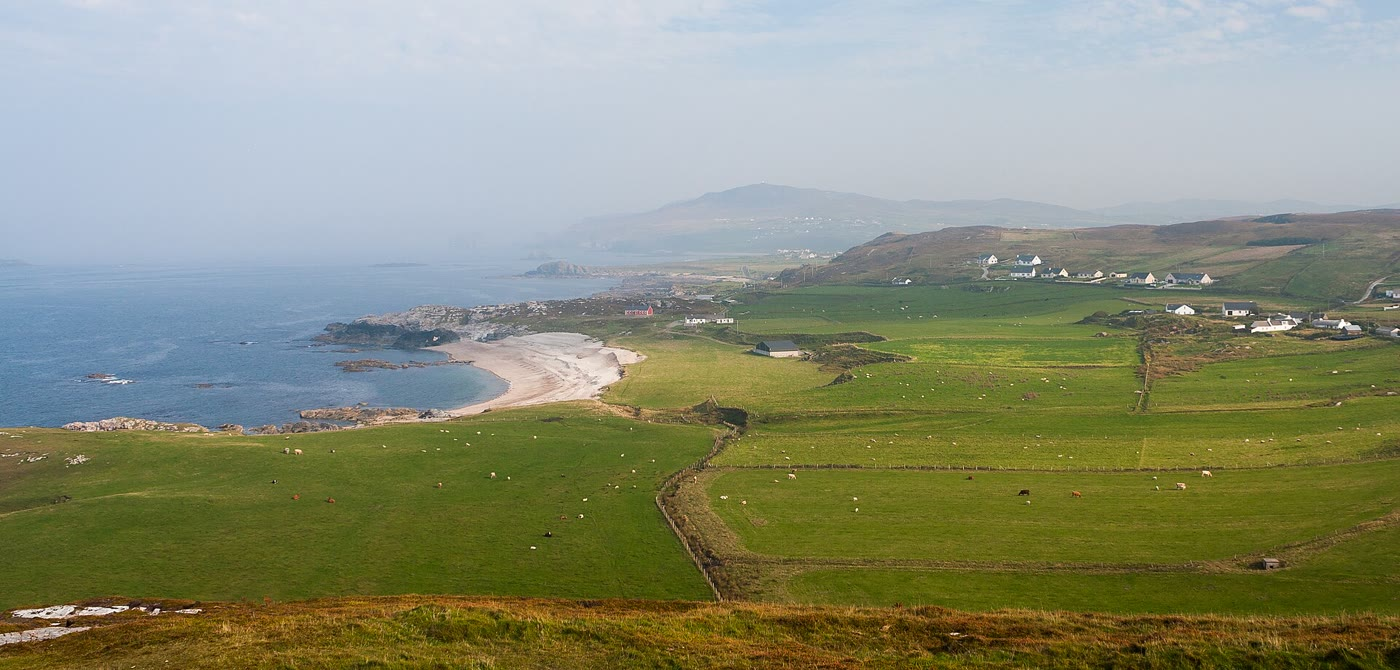
\includegraphics[width=\linewidth]{images/book5/b3-raised-beach-malin.jpg}

{\scriptsize Les plages soulevées de Ballyhillin, à Malin Head, dans le nord de l'Irlande~:
cordons de galets d'anciens rivages soulevés au-dessus de la mer à mesure que la terre
se soulevait après la fonte de sa calotte glaciaire. Photo A.~F.~Borchert, CC BY-SA 4.0.}
\end{minipage}
\end{inthefield}
% ledger: photo:b3-raised-beach

\section{Convection du manteau entier et sa structure profonde}

Le manteau convecte-t-il en une seule couche, ou en deux, au-dessus et au-dessous de la
discontinuité de \qty{670}{km}~? La tomographie (\cref{ch:b3:seismology-imaging})
apporte une réponse partielle~: certains panneaux plongeants s'aplatissent au-dessus de la discontinuité, d'autres plongent
à travers elle jusque dans le manteau inférieur, de sorte que de la matière la franchit et que les deux couches ne sont pas
isolées l'une de l'autre. L'augmentation de la viscosité avec la profondeur rend
l'écoulement du manteau inférieur plus lent, et les panneaux ralentissent et s'épaississent en y pénétrant.

À la base du manteau, la tomographie met en évidence deux vastes régions de faible vitesse des ondes S,
sous l'Afrique et sous le Pacifique, appelées grandes provinces à faible vitesse de cisaillement
(LLSVP). Elles sont vraisemblablement chimiquement distinctes du manteau situé au-dessus
d'elles et plus denses, formant des amas plutôt que des panaches chauds. Les grandes provinces magmatiques et
les kimberlites des dernières centaines de millions d'années ont surtout fait éruption au-dessus de leurs
bordures, comme si les panaches s'élevaient depuis les bords des amas, là où la couche limite
thermique chaude de la base du manteau vient les frôler.
% ledger: st12:llsvp

\section{Exercices}

\begin{exercise}[$\star$]\label{exo:b3:mantle-convection:1}
Calculer le \omterm{def:b3:mantle-convection:rayleigh}{nombre de Rayleigh} d'une couche du manteau supérieur de \qty{670}{km} d'épaisseur, avec
$\rho = \qty{3500}{kg.m^{-3}}$, $g = \qty{9.9}{m.s^{-2}}$, $\alpha =
\qty{3e-5}{K^{-1}}$, $\Delta T = \qty{1000}{K}$, $\kappa =
\qty{e-6}{m^2.s^{-1}}$ et $\eta = \qty{5e20}{Pa.s}$. Combien de fois est-il supérieur au nombre
critique, pour des limites à glissement libre~?
\end{exercise}

\begin{exercise}[$\star$]\label{exo:b3:mantle-convection:2}
Calculer le \omterm{def:b3:mantle-convection:maxwell}{temps de Maxwell} d'un manteau de viscosité \qty{e21}{Pa.s} et de
module de cisaillement \qty{7.7e10}{Pa}, en années. Le manteau répond-il de façon élastique ou visqueuse
à la marée terrestre semi-diurne, à la fonte d'une calotte glaciaire et à
l'enfoncement d'un panneau plongeant~?
\end{exercise}

\begin{exercise}[$\star$]\label{exo:b3:mantle-convection:3}
Avec $\eta = \qty{e21}{Pa.s}$, $\rho = \qty{3300}{kg.m^{-3}}$ et $g =
\qty{9.8}{m.s^{-2}}$, calculer le temps de relaxation d'un demi-espace uniforme pour
des charges de longueur d'onde 1000 et \qty{3000}{km}. Laquelle se rétablit le plus vite~?
\end{exercise}

\begin{exercise}[$\star$]\label{exo:b3:mantle-convection:4}
Avec $g = \qty{9.8}{m.s^{-2}}$, $\rho_m = \qty{3300}{kg.m^{-3}}$, $\rho_w =
\qty{1030}{kg.m^{-3}}$, $\alpha = \qty{3.1e-5}{K^{-1}}$, $T_m - T_0 =
\qty{1450}{K}$, $\kappa = \qty{0.8e-6}{m^2.s^{-1}}$ et \qty{1}{Ma} $=
\qty{3.156e13}{s}$, calculer la \omterm{prop:b3:mantle-convection:ridge-push}{force de poussée à la dorsale} à \qty{50}{Ma}. Combien de fois
plus petite est-elle que la traction du panneau plongeant de \qty{4.6e13}{N.m^{-1}}~?
\end{exercise}

\begin{exercise}[$\star\star$]\label{exo:b3:mantle-convection:5}
Une masse de manteau de \qty{10}{km} de diamètre, plus chaude de \qty{300}{K} que son
environnement, s'élève à la vitesse $\rho g\alpha\Delta Td^2/\eta$ (prendre $\rho =
\qty{3300}{kg.m^{-3}}$, $g = \qty{9.8}{m.s^{-2}}$, $\alpha = \qty{3e-5}{K^{-1}}$,
$\eta = \qty{e21}{Pa.s}$, $\kappa = \qty{e-6}{m^2.s^{-1}}$). (a) Calculer son
temps de montée sur sa propre taille et son temps de diffusion $d^2/\kappa$, et montrer que
leur rapport est son \omterm{def:b3:mantle-convection:rayleigh}{nombre de Rayleigh}. (b) Monte-t-elle ou se refroidit-elle d'abord~? (c)
Quelle doit être sa taille pour que son \omterm{def:b3:mantle-convection:rayleigh}{nombre de Rayleigh} atteigne 657.5~?
\end{exercise}

\begin{exercise}[$\star\star$]\label{exo:b3:mantle-convection:6}
Pour une couche de \qty{2891}{km} d'épaisseur, à $\mathrm{Ra} = \num{e7}$, avec $\kappa =
\qty{e-6}{m^2.s^{-1}}$, $k = \qty{3.1}{W.m^{-1}.K^{-1}}$, $\Delta T =
\qty{1450}{K}$ et $\mathrm{Ra}_c = 657.5$, calculer l'épaisseur de la couche
limite, le \omterm{def:b3:mantle-convection:nusselt}{nombre de Nusselt}, l'échelle de vitesse en \unit{cm/an} et le
flux de chaleur.
\end{exercise}

\begin{exercise}[$\star\star$]\label{exo:b3:mantle-convection:7}
Un renflement fictif associé à un point chaud a une section transversale de \qty{8e8}{m^2} à
travers la trace, et la plaque au-dessus se déplace à \qty{9}{cm/an}. Avec $\rho_m - \rho_w =
\qty{2270}{kg.m^{-3}}$, calculer son flux de flottabilité, et son flux de chaleur avec $c_p =
\qty{1170}{J.kg^{-1}.K^{-1}}$ et $\alpha = \qty{3.1e-5}{K^{-1}}$. Quelle fraction
des \qty{46.7}{TW} de la Terre représente-t-elle~?
\end{exercise}

\begin{exercise}[$\star\star$]\label{exo:b3:mantle-convection:8}
Une tête de panache de rayon \qty{400}{km}, plus légère que le manteau de
\qty{30}{kg.m^{-3}}, s'élève à travers un manteau de viscosité \qty{e21}{Pa.s}. Avec
la loi de Stokes, calculer sa vitesse en \unit{m/an} et le temps nécessaire pour parcourir
\qty{2000}{km}.
\end{exercise}

\begin{exercise}[$\star\star$]\label{exo:b3:mantle-convection:9}
Une région s'est enfoncée de \qty{300}{m} lorsque sa glace a fondu, il y a \qty{10}{ka},
et relaxe avec $\tau = \qty{4.4}{ka}$. Calculer l'enfoncement subsistant aujourd'hui et
le taux de soulèvement actuel. Comparer ce résultat au taux de \qty{10.3}{mm/an} mesuré près
d'Umeå.
\end{exercise}

\begin{exercise}[$\star\star\star$]\label{exo:b3:mantle-convection:10}
(a) À partir de l'expression de $F_{rp}$ dans la démonstration de
la \cref{prop:b3:mantle-convection:ridge-push}, montrer que le premier terme,
$\tfrac12(\rho_m - \rho_w)gw^2$, est le second terme du crochet. (b) Montrer que
$\int_0^\infty x\operatorname{erfc}x\,\mathrm dx = 1/4$, en intégrant par parties.
(c) Avec les valeurs de l'exercice 4, calculer les deux termes à \qty{100}{Ma}.
\end{exercise}

\begin{exercise}[$\star\star\star$]\label{exo:b3:mantle-convection:11}
Montrer que $f(k) = (\pi^2 + k^2)^3/k^2$ est minimale pour $k = \pi/\sqrt2$, où
elle vaut $27\pi^4/4$. En déduire la largeur d'une paire de cellules de convection au seuil,
en unités de $d$, et la largeur d'une seule cellule.
\end{exercise}

\begin{exercise}[$\star\star\star$]\label{exo:b3:mantle-convection:12}
Une plaque longue de \qty{6000}{km} se déplace à \qty{6}{cm/an} au-dessus
d'une couche du manteau de \qty{150}{km} d'épaisseur, de viscosité \qty{e20}{Pa.s}, dont la base est immobile. (a)
Calculer la \omterm{def:b3:mantle-convection:basal-drag}{traînée basale} en \unit{MPa} et la force de traînée par unité de longueur de plaque.
(b) Comparer avec une poussée à la dorsale de \qty{3.8e12}{N.m^{-1}} et une traction du panneau plongeant de
\qty{4.6e13}{N.m^{-1}}. (c) Si un dixième de la traction du panneau plongeant atteint la plaque,
à quelle vitesse la traînée équilibre-t-elle les forces motrices~?
\end{exercise}

\section{Problème~: rebond du lac Ardo}

\begin{problem}[{Problème du week-end --- le rebond du bassin d'un lac fictif,
la viscosité du manteau sous celui-ci, et la convection que cette viscosité
permet}]
\label{pb:b3:mantle-convection:1}
% values: calc/ch06.py; gia_relaxation.py, convection_scaling.py
Le lac Ardo, un lac fictif, remplissait un bassin large de \qty{250}{km}, barré par une
calotte glaciaire, et atteignait \qty{300}{m} de profondeur pendant environ cinquante mille ans. Il y a
quatorze mille ans, la digue de glace céda et le lac se vida en quelques semaines. Sa
plus haute ligne de rivage, horizontale lors de sa formation, est aujourd'hui inclinée~; des
rivages datés des petits lacs restés dans le bassin donnent le soulèvement du centre depuis la
vidange, par rapport à la bordure, qui a à peine bougé~:

\smallskip
\begin{center}\small
\begin{tabular}{lcccccc}
\hline
durée depuis la vidange (ka) & 1 & 2 & 4 & 6 & 9 & 14\\
soulèvement du centre (m) & 11.5 & 21.6 & 38.0 & 50.5 & 64.0 & 77.2\\
\hline
\end{tabular}
\end{center}
\smallskip

Prenez $\rho_w = \qty{1000}{kg.m^{-3}}$, $\rho_m = \qty{3300}{kg.m^{-3}}$, $g =
\qty{9.8}{m.s^{-2}}$, \qty{1}{an} $= \qty{3.156e7}{s}$, et traitez le manteau comme
un demi-espace visqueux homogène.

\medskip\noindent\textbf{Partie I --- La charge.}
\begin{enumerate}
  \item Calculer la pression exercée par le lac sur son fond.
  \item Calculer l'enfoncement du fond à l'équilibre isostatique, et dire
        pourquoi c'est la masse volumique du manteau, et non celle de la croûte, qui y intervient.
  \item En assimilant le lac à un disque, calculer la masse de son eau.
  \item Expliquer pourquoi la plus haute ligne de rivage est aujourd'hui inclinée, et calculer sa
        pente moyenne de la bordure au centre, en mètres par kilomètre.
  \item On traite l'enfoncement comme un harmonique unique dont la moitié déprimée, de
        $-\lambda/4$ à $\lambda/4$, couvre le lac. Donner $\lambda$ et $k =
        2\pi/\lambda$.
  \item Sur quelle profondeur l'écoulement sous une telle charge décroît-il d'un facteur
        $e$~?
\end{enumerate}

\medskip\noindent\textbf{Partie II --- Le temps de relaxation.}
\begin{enumerate}[resume]
  \item En supposant que le lac ait atteint l'équilibre, calculer l'enfoncement subsistant
        à chaque date du tableau.
  \item Montrer que, si l'enfoncement décroît exponentiellement, son logarithme décroît
        linéairement avec le temps.
  \item Calculer $\tau$ à partir des dates 1 et \qty{14}{ka}.
  \item Prévoir le soulèvement à \qty{6}{ka} avec ce $\tau$ et comparer avec le
        tableau.
  \item Calculer l'enfoncement subsistant aujourd'hui et le taux de soulèvement actuel du
        centre, en \unit{mm/an}.
  \item Quel soulèvement reste-t-il à venir~?
  \item Dans combien d'années encore le taux de soulèvement passera-t-il sous
        \qty{0.5}{mm/an}~?
\end{enumerate}

\medskip\noindent\textbf{Partie III --- La viscosité.}
\begin{enumerate}[resume]
  \item Calculer la viscosité du demi-espace à partir de $\tau$.
  \item La comparer aux \omterm{def:b3:mantle-convection:gia}{viscosités du manteau} supérieur, comprises entre \num{3.4e20} et
        \qty{1e21}{Pa.s} mesurées sous la Fennoscandie. Quelle partie du manteau
        le rebond du lac Ardo sonde-t-il~?
  \item Avec cette viscosité, calculer le temps de relaxation d'une charge
        de \qty{3000}{km} de longueur d'onde. Pourquoi une calotte glaciaire réelle de cette taille
        relaxerait-elle plus lentement que dans ce modèle~?
  \item Que fait une lithosphère élastique, négligée ici, au rebond
        d'une charge large de seulement \qty{250}{km}~?
  \item Calculer le \omterm{def:b3:mantle-convection:maxwell}{temps de Maxwell} du manteau avec $\mu = \qty{7.7e10}{Pa}$,
        et dire si un modèle visqueux était justifié.
  \item Vérifier l'hypothèse de la question~7~: quelle fraction de l'enfoncement d'équilibre
        a été atteinte pendant que le lac subsistait~?
  \item De combien varierait $\log_{10}\eta$ si l'on prenait $\lambda$ égal à
        \qty{250}{km}~?
\end{enumerate}

\medskip\noindent\textbf{Partie IV --- Convection.} Prenez une couche de manteau supérieur
\qty{670}{km} de profondeur, avec $\rho = \qty{3700}{kg.m^{-3}}$, $g =
\qty{9.9}{m.s^{-2}}$, $\alpha = \qty{3.1e-5}{K^{-1}}$, $\Delta T =
\qty{1450}{K}$, $\kappa = \qty{e-6}{m^2.s^{-1}}$, $k = \qty{3.1}{W.m^{-1}.K^{-1}}$
et la viscosité de la partie III.
\begin{enumerate}[resume]
  \item Calculer le \omterm{def:b3:mantle-convection:rayleigh}{nombre de Rayleigh} de la couche.
  \item De combien de fois le \omterm{def:b3:mantle-convection:rayleigh}{nombre de Rayleigh} dépasse-t-il le nombre critique ($\mathrm{Ra}_c = 657.5$)~?
  \item Calculer l'épaisseur de la couche limite et le \omterm{def:b3:mantle-convection:nusselt}{nombre de Nusselt}.
  \item Calculer l'échelle de vitesse en \unit{cm/an}, et la comparer aux vitesses de plaques
        de 1 à \qty{7.5}{cm/an}.
  \item Calculer le flux de chaleur, et donner deux raisons pour lesquelles il est inférieur à la
        valeur moyenne terrestre, \qty{92}{mW.m^{-2}}.
  \item Donner la \omterm{def:b3:mantle-convection:gia}{viscosité du manteau} supérieur sous le lac Ardo sous forme de $\log_{10}$ de
        $\eta$ en \unit{Pa.s}.
\end{enumerate}
\end{problem}
